\documentclass{article}



\usepackage{arxiv}

\usepackage[utf8]{inputenc} % allow utf-8 input
\usepackage[T1]{fontenc}    % use 8-bit T1 fonts
\usepackage{hyperref}       % hyperlinks
\usepackage{url}            % simple URL typesetting
\usepackage{booktabs}       % professional-quality tables
\usepackage{amsfonts}       % blackboard math symbols
\usepackage{nicefrac}       % compact symbols for 1/2, etc.
\usepackage{microtype}      % microtypography
\usepackage{lipsum}		% Can be removed after putting your text content
\usepackage{graphicx}
\usepackage{natbib}
\usepackage{doi}
\usepackage{float}

\usepackage{xcolor}
\hypersetup{
    colorlinks,
    linkcolor={red!50!black},
    citecolor={blue!50!black},
    urlcolor={blue!80!black}
}

\title{Scalable Computing Project 3 - P2P Computing with NDN for Hospital Patient Data Exchange}


\date{November, 2023}


\author{ 
{
\includegraphics[scale=0.2]{star.png}\hspace{1mm}
        Anupal Mishra	                     }\\
	<ID>          \\
	\texttt{shortname@tcd.ie}            \\
\And
{
\includegraphics[scale=0.2]{star.png}\hspace{1mm}
        Noêl Mathis	                 	 }\\
	23337722                          \\
	\texttt{mathisn@tcd.ie}            \\
\And
{
\includegraphics[scale=0.2]{star.png}\hspace{1mm}
        Nupur Rathod		             	 }\\
 	<ID>                                  \\
	\texttt{shortname@tcd.ie}            \\
\And
{
\includegraphics[scale=0.2]{star.png}\hspace{1mm}
        Frason Francis      	         	 }\\
	<ID>                                  \\
	\texttt{shortname@tcd.ie}            \\
}


\begin{document}
\maketitle
\section{Scenario and Ideas for Implementation}

\begin{figure}[H]
	\centering
        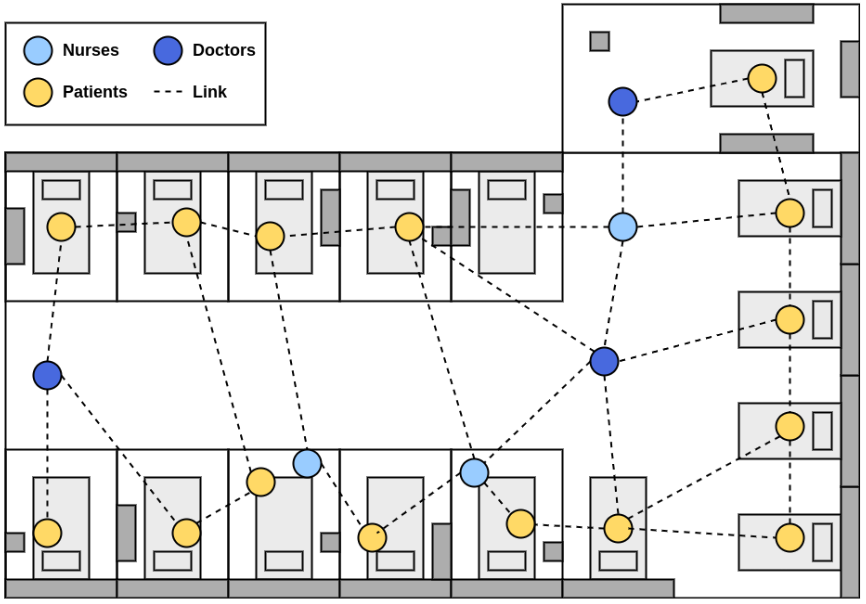
\includegraphics[scale=0.4]{media/scenario.png}
	\caption{Scenario}
	\label{fig:scenario_graphic}
\end{figure}




\bibliographystyle{unsrtnat}
\bibliography{references} 













%%% Uncomment this line and comment out the ``thebibliography'' section below to use the external .bib file (using bibtex) .


%%% Uncomment this section and comment out the \bibliography{references} line above to use inline references.
% \begin{thebibliography}{1}

% 	\bibitem{kour2014real}
% 	George Kour and Raid Saabne.
% 	\newblock Real-time segmentation of on-line handwritten arabic script.
% 	\newblock In {\em Frontiers in Handwriting Recognition (ICFHR), 2014 14th
% 			International Conference on}, pages 417--422. IEEE, 2014.

% 	\bibitem{kour2014fast}
% 	George Kour and Raid Saabne.
% 	\newblock Fast classification of handwritten on-line arabic characters.
% 	\newblock In {\em Soft Computing and Pattern Recognition (SoCPaR), 2014 6th
% 			International Conference of}, pages 312--318. IEEE, 2014.

% 	\bibitem{hadash2018estimate}
% 	Guy Hadash, Einat Kermany, Boaz Carmeli, Ofer Lavi, George Kour, and Alon
% 	Jacovi.
% 	\newblock Estimate and replace: A novel approach to integrating deep neural
% 	networks with existing applications.
% 	\newblock {\em arXiv preprint arXiv:1804.09028}, 2018.

% \end{thebibliography}


\end{document}
